% =====================================================================
%  NEURAX — The Analytical Compiler
%  Workshop deck. Scope: the compiler, and nothing else.
%
%  Build:  latexmk -pdf neurax-compiler.tex
%  Engine: pdflatex (no external assets — every figure is TikZ/PGFPlots)
% =====================================================================
\documentclass[aspectratio=169,11pt]{beamer}

\usetheme{default}
\usecolortheme{default}
\setbeamertemplate{navigation symbols}{}

% ── Fonts ────────────────────────────────────────────────────────────
\usepackage[T1]{fontenc}
\usepackage[utf8]{inputenc}
\usepackage{sourcesanspro}
\usepackage[scale=0.86]{sourcecodepro}
\usepackage{microtype}

% ── Figures ──────────────────────────────────────────────────────────
\usepackage{tikz}
\usepackage{pgfplots}
\pgfplotsset{compat=1.18}
\usetikzlibrary{arrows.meta,positioning,calc,fit,backgrounds,shapes.geometric,decorations.pathreplacing}
\usepackage{booktabs}
\usepackage{amsmath}

% ── Palette ──────────────────────────────────────────────────────────
% Chosen against a white ground: one deep structural blue carries the
% pipeline, one warm accent carries emphasis, and green/rose are reserved
% for "measured" and "refused" so colour always means something.
\definecolor{nxInk}   {HTML}{14171C}
\definecolor{nxSlate} {HTML}{57616F}
\definecolor{nxMute}  {HTML}{8A94A2}
\definecolor{nxDeep}  {HTML}{0E3D5E}
\definecolor{nxTeal}  {HTML}{16697A}
\definecolor{nxFlame} {HTML}{C2560B}
\definecolor{nxMoss}  {HTML}{1D7A52}
\definecolor{nxRose}  {HTML}{A81F45}
\definecolor{nxMist}  {HTML}{EEF2F5}
\definecolor{nxRule}  {HTML}{D8DFE6}

% The eleven phases, as one ramp: cool at the front end, warm at the
% report. The gradient is the argument — each pass lowers towards cost.
\definecolor{ph1}{HTML}{0E3D5E}
\definecolor{ph2}{HTML}{14506F}
\definecolor{ph3}{HTML}{176380}
\definecolor{ph4}{HTML}{1B7690}
\definecolor{ph5}{HTML}{2C8A8C}
\definecolor{ph6}{HTML}{5C9A6E}
\definecolor{ph7}{HTML}{8FA854}
\definecolor{ph8}{HTML}{BFAE3E}
\definecolor{ph9}{HTML}{D4913A}
\definecolor{ph10}{HTML}{C2560B}
\definecolor{ph11}{HTML}{8A3B12}

% ── Beamer colours: white ground, everywhere ─────────────────────────
\setbeamercolor{background canvas}{bg=white}
\setbeamercolor{normal text}{fg=nxInk}
\setbeamercolor{structure}{fg=nxDeep}
\setbeamercolor{frametitle}{fg=nxInk,bg=white}
\setbeamercolor{title}{fg=nxInk}
\setbeamercolor{itemize item}{fg=nxFlame}
\setbeamercolor{itemize subitem}{fg=nxMute}
\setbeamercolor{alerted text}{fg=nxFlame}
\setbeamerfont{frametitle}{size=\Large,series=\bfseries}
\setbeamerfont{framesubtitle}{size=\small,series=\mdseries}
\setbeamercolor{framesubtitle}{fg=nxSlate}
\setbeamertemplate{itemize item}{\raisebox{0.12ex}{\scriptsize$\blacktriangleright$}}
\setbeamertemplate{itemize subitem}{\raisebox{0.15ex}{\tiny$\bullet$}}

% Frame title: a name, a thin rule, room to breathe.
\makeatletter
\setbeamertemplate{frametitle}{%
  \vspace{0.6em}%
  \begin{minipage}{\textwidth}
    \raggedright\usebeamerfont{frametitle}\usebeamercolor[fg]{frametitle}\insertframetitle\par
    \ifx\insertframesubtitle\@empty\else
      \vspace{0.15em}\usebeamerfont{framesubtitle}\usebeamercolor[fg]{framesubtitle}\insertframesubtitle\par
    \fi
    \vspace{0.35em}\textcolor{nxRule}{\rule{\linewidth}{0.6pt}}
  \end{minipage}%
  \vspace{0.2em}%
}
\makeatother

% Footline: section, and a page number that is not shouting.
\setbeamertemplate{footline}{%
  \hbox{\begin{beamercolorbox}[wd=\paperwidth,ht=2.4ex,dp=1.4ex,leftskip=1.1em,rightskip=1.1em]{}%
    {\scriptsize\color{nxMute}\textsc{neurax}\hfill\insertsectionhead\hfill\insertframenumber}%
  \end{beamercolorbox}}%
}

% Content must never reach the footline. Beamer will not tell you when it
% does — it just draws over it — so the margin is enforced here rather
% than remembered slide by slide.
\setbeamersize{text margin left=1.0em,text margin right=1.0em}
\addtobeamertemplate{frametitle}{}{\vspace{-0.15em}}

% ── Small helpers ────────────────────────────────────────────────────
% Size-neutral on purpose: an absolute \small here made code *bigger*
% than the \tiny caption around it, which is exactly backwards.
\newcommand{\code}[1]{\texttt{\color{nxDeep}#1}}
\newcommand{\term}[1]{\textcolor{nxFlame}{\textbf{#1}}}
\newcommand{\good}[1]{\textcolor{nxMoss}{#1}}
\newcommand{\bad}[1]{\textcolor{nxRose}{#1}}
\newcommand{\subtle}[1]{{\footnotesize\color{nxSlate}#1}}

% A quiet callout box, for the one sentence that matters on a slide.
\newcommand{\keypoint}[1]{%
  \begin{tikzpicture}
    \node[fill=nxMist,text=nxInk,rounded corners=2pt,inner sep=8pt,
          text width=\dimexpr\linewidth-20pt\relax,align=left] {#1};
  \end{tikzpicture}%
}

\newcommand{\phasebadge}[2]{%
  \tikz[baseline=-0.5ex]{\node[fill=#1,text=white,rounded corners=1.5pt,
        inner xsep=4pt,inner ysep=1.6pt,font=\scriptsize\bfseries]{#2};}%
}

\title{\textbf{NEURAX}}
\subtitle{An analytical compiler for neural network architectures}
\date{}

% =====================================================================
\begin{document}

% ── Title ────────────────────────────────────────────────────────────
\begin{frame}[plain]
  \vspace{1.1cm}
  
\begin{tikzpicture}[remember picture]
    \node[anchor=west,inner sep=0] (t) at (0,0)
      {\fontsize{34}{38}\selectfont\bfseries\color{nxInk}NEURAX};
    \node[anchor=west,inner sep=0,below=6pt of t.south west]
      {\fontsize{15}{19}\selectfont\color{nxDeep}The analytical compiler};
  \end{tikzpicture}

  \vspace{0.9cm}
  {\large\color{nxSlate}What a neural network will cost,\\[2pt]
   derived from its architecture --- without running it.}

  \vspace{1.0cm}
  \textcolor{nxRule}{\rule{0.42\linewidth}{0.8pt}}

  \vspace{0.4cm}
  {\footnotesize\color{nxMute}
   Eleven dialects, from a JSON description to a costed report.\\
   This talk is about the compiler, and only the compiler.}
\end{frame}

% ── Scope ────────────────────────────────────────────────────────────
\begin{frame}{What this talk covers}{And, deliberately, what it does not}
  \vspace{0.2cm}
  \begin{columns}[T]
    \begin{column}{0.47\textwidth}
      {\color{nxMoss}\bfseries In scope}\\[6pt]
      \textcolor{nxRule}{\rule{\linewidth}{0.6pt}}\\[8pt]
      \begin{itemize}\setlength\itemsep{5pt}
        \item The intermediate representation and its eleven passes
        \item How parameters, FLOPs, memory, latency and cost are derived
        \item The analytical formula library
        \item How the results are validated against published models
        \item Where the model is approximate, and by how much
      \end{itemize}
    \end{column}
    \begin{column}{0.47\textwidth}
      {\color{nxMute}\bfseries Out of scope}\\[6pt]
      \textcolor{nxRule}{\rule{\linewidth}{0.6pt}}\\[8pt]
      \begin{itemize}\setlength\itemsep{5pt}
        \color{nxSlate}
        \item The visual studio and its workspaces
        \item Hardware detection and measurement
        \item The training runtime
        \item Code generation
        \item The assistant
      \end{itemize}
      \vspace{10pt}
      \subtle{Each is a talk of its own. The compiler is the part every one of
      them is built on top of.}
    \end{column}
  \end{columns}
\end{frame}

% =====================================================================
\section{The problem}
% =====================================================================

\begin{frame}{The question}{Asked before the money is spent, not after}
  \vspace{0.35cm}
  \begin{center}
  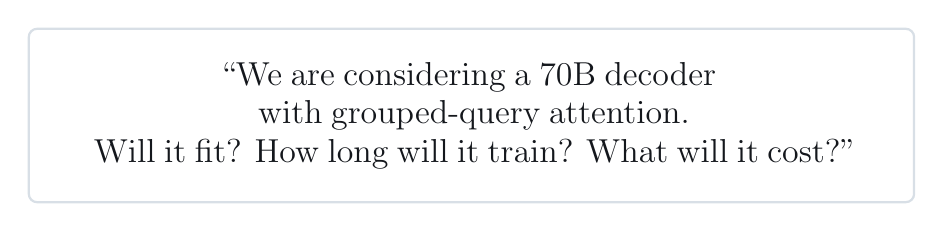
\begin{tikzpicture}[font=\small]
    \node[draw=nxRule,fill=white,rounded corners=3pt,inner sep=12pt,
          text width=10.4cm,align=center,line width=0.8pt]
      {\large\color{nxInk}
       ``We are considering a 70B decoder with grouped-query attention.\\[3pt]
        Will it fit? How long will it train? What will it cost?''};
  \end{tikzpicture}
  \end{center}

  \vspace{0.55cm}
  \begin{columns}[T]
    \begin{column}{0.31\textwidth}
      \phasebadge{nxRose}{TODAY}\\[7pt]
      {\bfseries Run a smaller version}\\[3pt]
      \subtle{Hours of GPU time to answer a question about a model you did not
      build. Extrapolating from it is a second guess on top of the first.}
    \end{column}
    \begin{column}{0.31\textwidth}
      \phasebadge{nxRose}{TODAY}\\[7pt]
      {\bfseries Ask someone who has}\\[3pt]
      \subtle{Fast, unreproducible, and specific to their hardware, their batch
      size and their framework version.}
    \end{column}
    \begin{column}{0.31\textwidth}
      \phasebadge{nxMoss}{NEURAX}\\[7pt]
      {\bfseries Derive it}\\[3pt]
      \subtle{The cost of a network is a function of its shape. Shapes are known
      before any weight exists.}
    \end{column}
  \end{columns}
\end{frame}

\begin{frame}{Measure or derive}{Two answers to the same question, with very different economics}
  \vspace{0.3cm}
  \begin{center}
  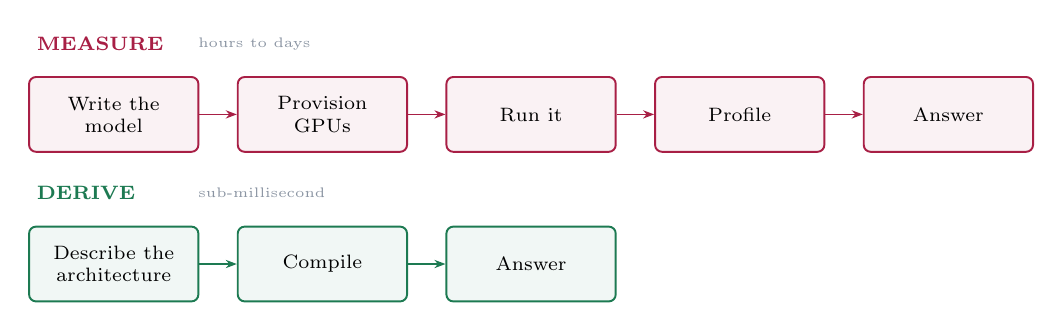
\begin{tikzpicture}[font=\footnotesize,
      box/.style={draw,rounded corners=2.5pt,minimum height=0.95cm,
                  minimum width=2.15cm,align=center,line width=0.7pt,
                  font=\scriptsize}]

    % MEASURE — five steps, and every one of them costs something
    \node[text=nxRose,font=\scriptsize\bfseries,anchor=west] at (0,2.62) {MEASURE};
    \node[text=nxMute,font=\tiny,anchor=west] at (2.05,2.62) {hours to days};
    \node[box,draw=nxRose,fill=nxRose!6] (m1) at (1.10,1.72) {Write the\\model};
    \node[box,draw=nxRose,fill=nxRose!6] (m2) at (3.75,1.72) {Provision\\GPUs};
    \node[box,draw=nxRose,fill=nxRose!6] (m3) at (6.40,1.72) {Run it};
    \node[box,draw=nxRose,fill=nxRose!6] (m4) at (9.05,1.72) {Profile};
    \node[box,draw=nxRose,fill=nxRose!6] (m5) at (11.70,1.72) {Answer};
    \foreach \a/\b in {m1/m2,m2/m3,m3/m4,m4/m5}
      \draw[-{Stealth[length=4pt]},nxRose] (\a) -- (\b);

    % DERIVE — the same answer, two steps earlier
    \node[text=nxMoss,font=\scriptsize\bfseries,anchor=west] at (0,0.72) {DERIVE};
    \node[text=nxMute,font=\tiny,anchor=west] at (2.05,0.72) {sub-millisecond};
    \node[box,draw=nxMoss,fill=nxMoss!6] (d1) at (1.10,-0.18) {Describe the\\architecture};
    \node[box,draw=nxMoss,fill=nxMoss!6] (d2) at (3.75,-0.18) {Compile};
    \node[box,draw=nxMoss,fill=nxMoss!6] (d3) at (6.40,-0.18) {Answer};
    \foreach \a/\b in {d1/d2,d2/d3}
      \draw[-{Stealth[length=4pt]},nxMoss] (\a) -- (\b);
  \end{tikzpicture}
  \end{center}

  \vspace{0.2cm}
  \keypoint{The measured answer is the ground truth --- and it is only
  available \emph{after} you have already paid for it. NEURAX gives up
  exactness to answer the question while it is still a question.}
\end{frame}

\begin{frame}{What an analytical compiler is}{The contract, stated plainly}
  \vspace{0.25cm}
  \begin{columns}[T]
    \begin{column}{0.53\textwidth}
      {\bfseries It takes} a description of an architecture: layer types,
      shapes, hyperparameters, a target device.\\[10pt]
      {\bfseries It returns} parameters, FLOPs, peak memory, latency,
      throughput, scaling behaviour, energy and money.\\[10pt]
      {\bfseries It never executes the model.} No tensor is allocated, no
      kernel is launched, no weight exists.\\[10pt]
      \subtle{Everything it reports is derived from the shape of the computation
      and a table of hardware constants.}
    \end{column}
    \begin{column}{0.43\textwidth}
      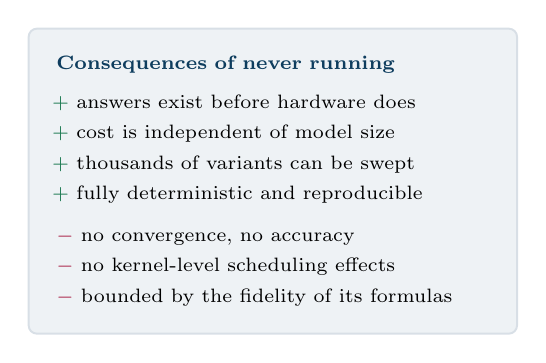
\begin{tikzpicture}[font=\scriptsize]
        \node[draw=nxRule,fill=nxMist,rounded corners=3pt,inner sep=10pt,
              text width=5.5cm,align=left,line width=0.7pt] {
          \textbf{\color{nxDeep}Consequences of never running}\\[6pt]
          \good{$+$} answers exist before hardware does\\[3pt]
          \good{$+$} cost is independent of model size\\[3pt]
          \good{$+$} thousands of variants can be swept\\[3pt]
          \good{$+$} fully deterministic and reproducible\\[7pt]
          \bad{$-$} no convergence, no accuracy\\[3pt]
          \bad{$-$} no kernel-level scheduling effects\\[3pt]
          \bad{$-$} bounded by the fidelity of its formulas
        };
      \end{tikzpicture}
    \end{column}
  \end{columns}
\end{frame}

% =====================================================================
\section{Structure}
% =====================================================================

\begin{frame}{How the compiler is built}{Five crates, one direction of dependency}
  \vspace{0.4cm}
  \begin{center}
  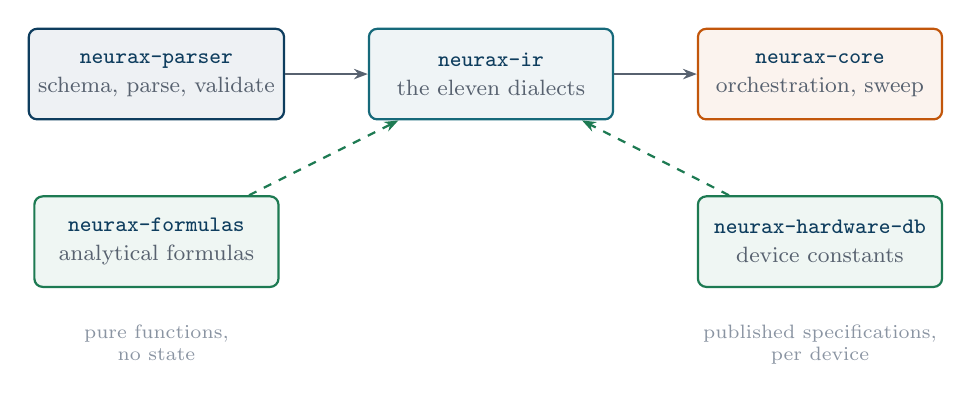
\begin{tikzpicture}[font=\footnotesize,
      crate/.style={draw,rounded corners=3pt,minimum width=3.1cm,
                    minimum height=1.15cm,align=center,line width=0.8pt}]

    \node[crate,draw=nxDeep,fill=nxDeep!7] (parser) at (0,0)
      {\textbf{\code{neurax-parser}}\\[1pt]\color{nxSlate}schema, parse, validate};
    \node[crate,draw=nxTeal,fill=nxTeal!7,right=1.05cm of parser] (ir)
      {\textbf{\code{neurax-ir}}\\[1pt]\color{nxSlate}the eleven dialects};
    \node[crate,draw=nxFlame,fill=nxFlame!7,right=1.05cm of ir] (core)
      {\textbf{\code{neurax-core}}\\[1pt]\color{nxSlate}orchestration, sweep};

    \node[crate,draw=nxMoss,fill=nxMoss!7,below=0.95cm of parser] (formulas)
      {\textbf{\code{neurax-formulas}}\\[1pt]\color{nxSlate}analytical formulas};
    \node[crate,draw=nxMoss,fill=nxMoss!7,below=0.95cm of core] (db)
      {\textbf{\code{neurax-hardware-db}}\\[1pt]\color{nxSlate}device constants};

    \draw[-{Stealth[length=5pt]},nxSlate,line width=0.8pt] (parser) -- (ir);
    \draw[-{Stealth[length=5pt]},nxSlate,line width=0.8pt] (ir) -- (core);
    \draw[-{Stealth[length=5pt]},nxMoss,line width=0.8pt,dashed] (formulas) -- (ir);
    \draw[-{Stealth[length=5pt]},nxMoss,line width=0.8pt,dashed] (db) -- (ir);

    \node[below=0.35cm of formulas,text=nxMute,font=\scriptsize,align=center]
      {pure functions,\\no state};
    \node[below=0.35cm of db,text=nxMute,font=\scriptsize,align=center]
      {published specifications,\\per device};
  \end{tikzpicture}
  \end{center}

  \vspace{0.35cm}
  \subtle{The two dashed crates are leaves: they know nothing about the pipeline,
  which is what makes each of them testable against published figures on its
  own. \code{neurax-formulas} is a library of pure functions --- given the same
  shape, it returns the same count, forever.}
\end{frame}

\begin{frame}{The front end}{Before any analysis, a description that is known to be well-formed}
  \vspace{0.2cm}
  \begin{columns}[T]
    \begin{column}{0.5\textwidth}
      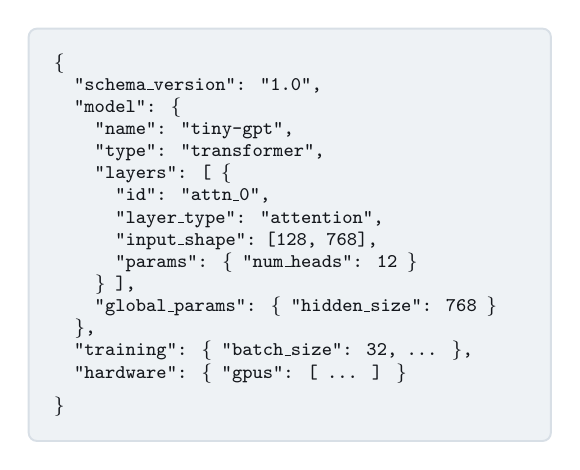
\begin{tikzpicture}
        \node[draw=nxRule,fill=nxMist,rounded corners=3pt,inner sep=9pt,
              text width=6.0cm,line width=0.7pt] {
          {\scriptsize\ttfamily\color{nxInk}
          \{\\
          \hspace*{1em}"schema\_version": "1.0",\\
          \hspace*{1em}"model": \{\\
          \hspace*{2em}"name": "tiny-gpt",\\
          \hspace*{2em}"type": "transformer",\\
          \hspace*{2em}"layers": [ \{\\
          \hspace*{3em}"id": "attn\_0",\\
          \hspace*{3em}"layer\_type": "attention",\\
          \hspace*{3em}"input\_shape":\ [128, 768],\\
          \hspace*{3em}"params": \{ "num\_heads": 12 \}\\
          \hspace*{2em}\} ],\\
          \hspace*{2em}"global\_params": \{ "hidden\_size": 768 \}\\
          \hspace*{1em}\},\\
          \hspace*{1em}"training": \{ "batch\_size": 32, ... \},\\
          \hspace*{1em}"hardware": \{ "gpus": [ ... ] \}\\
          \}}
        };
      \end{tikzpicture}
    \end{column}
    \begin{column}{0.46\textwidth}
      {\bfseries Three inputs, not one}\\[5pt]
      \subtle{A model is not costable on its own. The same architecture on a
      different device, at a different batch size, is a different answer ---
      so the device and the training regime are part of the input, not
      an afterthought.}\\[11pt]

      {\bfseries Validation rejects before it analyses}\\[5pt]
      \subtle{Zero attention heads, a hidden size that is not divisible by the
      head count, shapes that cannot connect. A compiler that produced a
      confident number for an impossible model would be worse than one that
      refused.}\\[11pt]

      \keypoint{\footnotesize Every downstream pass may assume its input is
      structurally sound. That assumption is what lets the formulas stay
      formulas.}
    \end{column}
  \end{columns}
\end{frame}

% =====================================================================
\section{The pipeline}
% =====================================================================

\begin{frame}{The pipeline}{Eleven dialects, each lowering the description one step closer to money}
  \vspace{0.1cm}
  \begin{center}
  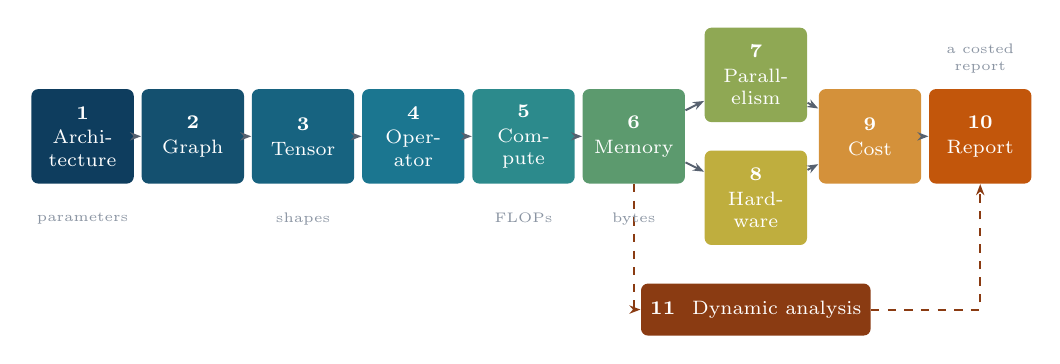
\begin{tikzpicture}[font=\scriptsize,
      ph/.style={draw=none,rounded corners=2.5pt,text=white,
                 minimum width=1.30cm,minimum height=1.20cm,align=center,
                 font=\scriptsize\bfseries}]

    \node[ph,fill=ph1]  (p1)  at (0.00,0) {1\\[1pt]\mdseries Archi-\\\mdseries tecture};
    \node[ph,fill=ph2]  (p2)  at (1.40,0) {2\\[1pt]\mdseries Graph};
    \node[ph,fill=ph3]  (p3)  at (2.80,0) {3\\[1pt]\mdseries Tensor};
    \node[ph,fill=ph4]  (p4)  at (4.20,0) {4\\[1pt]\mdseries Oper-\\\mdseries ator};
    \node[ph,fill=ph5]  (p5)  at (5.60,0) {5\\[1pt]\mdseries Com-\\\mdseries pute};
    \node[ph,fill=ph6]  (p6)  at (7.00,0) {6\\[1pt]\mdseries Memory};
    \node[ph,fill=ph7]  (p7)  at (8.55,0.78) {7\\[1pt]\mdseries Parall-\\\mdseries elism};
    \node[ph,fill=ph8]  (p8)  at (8.55,-0.78) {8\\[1pt]\mdseries Hard-\\\mdseries ware};
    \node[ph,fill=ph9]  (p9)  at (10.00,0) {9\\[1pt]\mdseries Cost};
    \node[ph,fill=ph10] (p10) at (11.40,0) {10\\[1pt]\mdseries Report};

    \foreach \a/\b in {p1/p2,p2/p3,p3/p4,p4/p5,p5/p6}
      \draw[-{Stealth[length=4pt]},nxSlate,line width=0.7pt] (\a) -- (\b);
    \draw[-{Stealth[length=4pt]},nxSlate,line width=0.7pt] (p6) -- (p7);
    \draw[-{Stealth[length=4pt]},nxSlate,line width=0.7pt] (p6) -- (p8);
    \draw[-{Stealth[length=4pt]},nxSlate,line width=0.7pt] (p7) -- (p9);
    \draw[-{Stealth[length=4pt]},nxSlate,line width=0.7pt] (p8) -- (p9);
    \draw[-{Stealth[length=4pt]},nxSlate,line width=0.7pt] (p9) -- (p10);

    % The report is the output, named inside the canvas rather than hanging
    % off its right edge where the slide clipped it.
    \node[text=nxMute,font=\tiny,align=center,above=2pt of p10]
      {a costed\\report};

    \node[ph,fill=ph11,minimum width=2.9cm,minimum height=0.66cm]
      (p11) at (8.55,-2.20) {11\ \ \mdseries Dynamic analysis};
    \draw[-{Stealth[length=4pt]},ph11,line width=0.7pt,dashed] (p6.south) |- (p11.west);
    \draw[-{Stealth[length=4pt]},ph11,line width=0.7pt,dashed] (p11.east) -| (p10.south);

    % What is actually flowing along the pipe, under the pass that emits it.
    \node[below=0.24cm of p1,text=nxMute,align=center,font=\tiny] {parameters};
    \node[below=0.24cm of p3,text=nxMute,align=center,font=\tiny] {shapes};
    \node[below=0.24cm of p5,text=nxMute,align=center,font=\tiny] {FLOPs};
    \node[below=0.24cm of p6,text=nxMute,align=center,font=\tiny] {bytes};
  \end{tikzpicture}
  \end{center}

  \vspace{0.15cm}
  \keypoint{Each pass owns one question and may only read what the passes
  before it produced. Nothing reaches back --- which is what makes an
  eleven-stage derivation auditable: every number has exactly one place it
  could have come from.}
\end{frame}

\begin{frame}{The contract every pass signs}{Three methods, and the third is the interesting one}
  \vspace{0.2cm}
  \begin{columns}[T]
    \begin{column}{0.54\textwidth}
      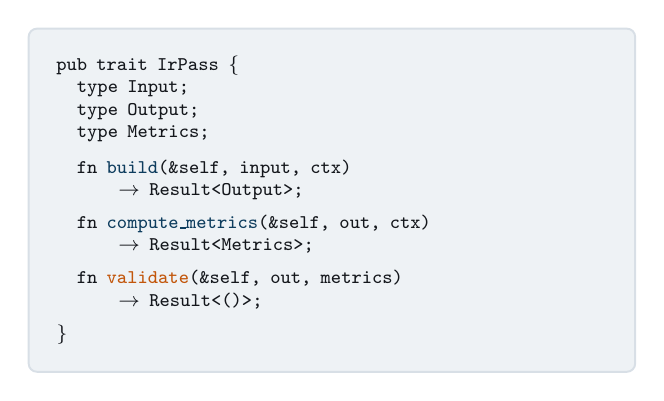
\begin{tikzpicture}
        \node[draw=nxRule,fill=nxMist,rounded corners=3pt,inner sep=10pt,
              text width=7.0cm,line width=0.7pt] {
          {\scriptsize\ttfamily\color{nxInk}
          pub trait IrPass \{\\
          \hspace*{1em}type Input;\\
          \hspace*{1em}type Output;\\
          \hspace*{1em}type Metrics;\\[5pt]
          \hspace*{1em}fn \textcolor{nxDeep}{\textbf{build}}(\&self, input, ctx)\\
          \hspace*{3em}$\rightarrow$ Result<Output>;\\[4pt]
          \hspace*{1em}fn \textcolor{nxDeep}{\textbf{compute\_metrics}}(\&self, out, ctx)\\
          \hspace*{3em}$\rightarrow$ Result<Metrics>;\\[4pt]
          \hspace*{1em}fn \textcolor{nxFlame}{\textbf{validate}}(\&self, out, metrics)\\
          \hspace*{3em}$\rightarrow$ Result<()>;\\
          \}}
        };
      \end{tikzpicture}
    \end{column}
    \begin{column}{0.42\textwidth}
      \term{build} lowers the previous dialect into this one.\\[9pt]
      \term{compute\_metrics} derives this pass's numbers from the lowered
      form.\\[9pt]
      \term{validate} checks them \emph{before} they are allowed downstream ---
      peak memory greater than zero, forward FLOPs greater than zero, shapes
      that connect.\\[12pt]
      \keypoint{\footnotesize A wrong number caught in the pass that produced it
      names that pass. The same number caught three passes later names nothing,
      and looks like a cost bug.}
    \end{column}
  \end{columns}
\end{frame}

% =====================================================================
\section{The passes}
% =====================================================================

\begin{frame}{Phases 1--2: Architecture and Graph}{From a list of layers to a directed acyclic graph}
  \vspace{0.2cm}
  \begin{columns}[T]
    \begin{column}{0.44\textwidth}
      \phasebadge{ph1}{PHASE 1}\ \ {\bfseries Architecture}\\[6pt]
      \subtle{Normalises the description into typed layer definitions and resolves
      repetition: a decoder stated as ``32 identical blocks'' becomes 32 blocks
      with real widths.}\\[4pt]
      \subtle{\textbf{Produces:} total parameters, layer count.}\\[13pt]

      \phasebadge{ph2}{PHASE 2}\ \ {\bfseries Graph}\\[6pt]
      \subtle{Builds the computational DAG, checks it is acyclic, and finds the
      critical path --- the longest chain of dependent operations, which is what
      bounds latency no matter how much hardware you add.}\\[4pt]
      \subtle{\textbf{Produces:} graph depth, operation count.}
    \end{column}
    \begin{column}{0.52\textwidth}
      \begin{center}
      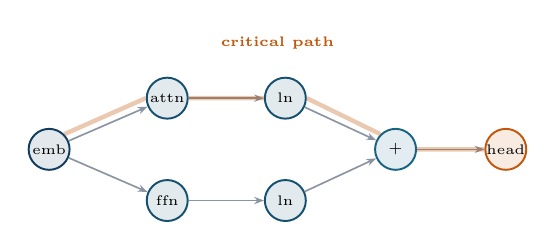
\begin{tikzpicture}[font=\tiny,
          n/.style={draw,circle,minimum size=0.52cm,inner sep=0,line width=0.7pt},
          e/.style={-{Stealth[length=3.5pt]},nxMute,line width=0.6pt}]
        \node[n,draw=ph1,fill=ph1!12] (emb) at (0,0) {emb};
        \node[n,draw=ph2,fill=ph2!12] (att) at (1.5,0.65) {attn};
        \node[n,draw=ph2,fill=ph2!12] (ln1) at (3.0,0.65) {ln};
        \node[n,draw=ph2,fill=ph2!12] (ffn) at (1.5,-0.65) {ffn};
        \node[n,draw=ph2,fill=ph2!12] (ln2) at (3.0,-0.65) {ln};
        \node[n,draw=ph3,fill=ph3!12] (add) at (4.4,0) {$+$};
        \node[n,draw=ph10,fill=ph10!12] (out) at (5.8,0) {head};

        \draw[e] (emb) -- (att); \draw[e] (emb) -- (ffn);
        \draw[e] (att) -- (ln1); \draw[e] (ffn) -- (ln2);
        \draw[e] (ln1) -- (add); \draw[e] (ln2) -- (add);
        \draw[e] (add) -- (out);

        \draw[nxFlame,line width=1.6pt,opacity=0.32]
          (emb.north east) -- (att.west) (att.east) -- (ln1.west)
          (ln1.east) -- (add.north west) (add.east) -- (out.west);
        \node[text=nxFlame,font=\tiny\bfseries] at (2.9,1.35) {critical path};
      \end{tikzpicture}
      \end{center}
      \vspace{0.35cm}
      \subtle{Fifty-five layer types are recognised, across transformers, CNNs,
      state-space models, mixtures of experts, RNNs, GNNs, GANs and diffusion.}
    \end{column}
  \end{columns}
\end{frame}

\begin{frame}{Phase 3: Tensor}{Shape inference --- every intermediate tensor, before any of them exists}
  \vspace{0.25cm}
  \begin{center}
  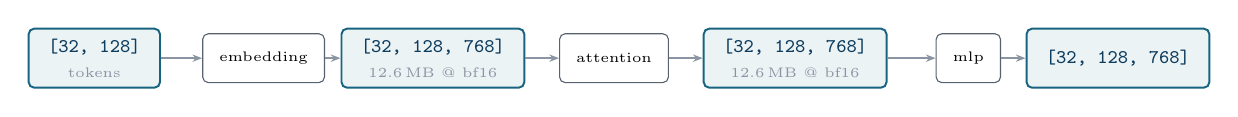
\begin{tikzpicture}[font=\scriptsize,
      t/.style={draw,rounded corners=2pt,minimum height=0.75cm,
                inner xsep=7pt,align=center,line width=0.7pt},
      op/.style={draw=nxSlate,fill=white,rounded corners=2pt,
                 minimum height=0.62cm,inner xsep=6pt,font=\tiny}]

    \node[t,draw=ph3,fill=ph3!8] (x0) at (0,0) {\code{[32, 128]}\\[1pt]\color{nxMute}\tiny tokens};
    \node[op] (o1) at (2.15,0) {embedding};
    \node[t,draw=ph3,fill=ph3!8] (x1) at (4.3,0) {\code{[32, 128, 768]}\\[1pt]\color{nxMute}\tiny 12.6\,MB @ bf16};
    \node[op] (o2) at (6.6,0) {attention};
    \node[t,draw=ph3,fill=ph3!8] (x2) at (8.9,0) {\code{[32, 128, 768]}\\[1pt]\color{nxMute}\tiny 12.6\,MB @ bf16};
    \node[op] (o3) at (11.1,0) {mlp};
    \node[t,draw=ph3,fill=ph3!8] (x3) at (13.0,0) {\code{[32, 128, 768]}};

    \foreach \a/\b in {x0/o1,o1/x1,x1/o2,o2/x2,x2/o3,o3/x3}
      \draw[-{Stealth[length=3.5pt]},nxMute,line width=0.6pt] (\a) -- (\b);
  \end{tikzpicture}
  \end{center}

  \vspace{0.5cm}
  \begin{columns}[T]
    \begin{column}{0.48\textwidth}
      {\bfseries Why shapes come before everything}\\[5pt]
      \subtle{A FLOP count is a function of the shapes a kernel operates on. A
      byte count is a function of the shapes that are live. Neither question can
      be asked until every intermediate shape is known.}
    \end{column}
    \begin{column}{0.48\textwidth}
      {\bfseries Where it refuses}\\[5pt]
      \subtle{If two shapes cannot connect, this is the pass that says so, naming
      the two layers. The alternative --- silently reshaping --- would produce a
      complete, confident and entirely fictional report.}
    \end{column}
  \end{columns}
\end{frame}

\begin{frame}{Phase 4: Operator}{From layers to the operations a device actually issues}
  \vspace{0.35cm}
  \begin{center}
  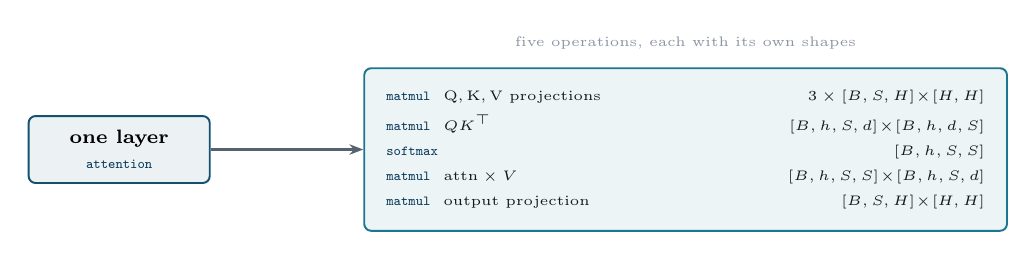
\begin{tikzpicture}[font=\scriptsize]
    \node[draw=ph2,fill=ph2!8,rounded corners=2.5pt,minimum height=0.85cm,
          minimum width=2.3cm,align=center,line width=0.7pt] (l) at (0,0)
      {\textbf{one layer}\\[1pt]\tiny\color{nxSlate}\code{attention}};

    \node[draw=ph4,fill=ph4!8,rounded corners=2.5pt,line width=0.7pt,
          inner sep=8pt,anchor=west] (ops) at (3.1,0) {%
      \begin{minipage}{7.6cm}\tiny\color{nxInk}
        \code{matmul}\ \ Q,\,K,\,V projections \hfill $3 \times [B,S,H]\!\times\![H,H]$\\[3pt]
        \code{matmul}\ \ $QK^{\top}$ \hfill $[B,h,S,d]\!\times\![B,h,d,S]$\\[3pt]
        \code{softmax} \hfill $[B,h,S,S]$\\[3pt]
        \code{matmul}\ \ $\text{attn}\times V$ \hfill $[B,h,S,S]\!\times\![B,h,S,d]$\\[3pt]
        \code{matmul}\ \ output projection \hfill $[B,S,H]\!\times\![H,H]$
      \end{minipage}};

    \draw[-{Stealth[length=5pt]},nxSlate,line width=0.8pt] (l) -- (ops);
    \node[above=3pt of ops,text=nxMute,font=\tiny]
      {five operations, each with its own shapes};
  \end{tikzpicture}
  \end{center}

  \vspace{0.4cm}
  \keypoint{This is the pass that makes the rest arithmetic. ``An attention
  layer'' has no FLOP count; five matmuls of known shape do. Fusion
  opportunities are identified here too --- adjacent elementwise operations a
  real kernel would not round-trip through memory.}
\end{frame}

\begin{frame}{Phase 5: Compute}{FLOPs, derived --- shown for attention, because it is the one that surprises}
  \vspace{0.15cm}
  \begin{columns}[T]
    \begin{column}{0.52\textwidth}
      \vspace{0.1cm}
      {\footnotesize
      \begin{align*}
        \text{QKV} &= 3 \cdot 2BSH\,w &
        QK^{\top}  &= 2Bh S^2 d \\[3pt]
        \text{attn}\!\cdot\!V &= 2Bh S^2 d &
        \text{softmax} &\approx 5\,Bh S^2 \\[3pt]
        \text{out}  &= 2BS\,wH
      \end{align*}}

      \vspace{0.2cm}
      \subtle{$B$ batch, $S$ sequence, $H$ hidden, $h$ heads, $d$ head
      dimension, $w = h\cdot d$.}

      \vspace{0.25cm}
      \subtle{Causal attention halves the three $S^2$ terms --- and only
      those three, because the projections are not masked.}

      \vspace{0.25cm}
      \subtle{Backward is taken as $2\times$ forward; the optimizer step adds
      $\approx 10\%$.}
    \end{column}
    \begin{column}{0.46\textwidth}
      \begin{center}
      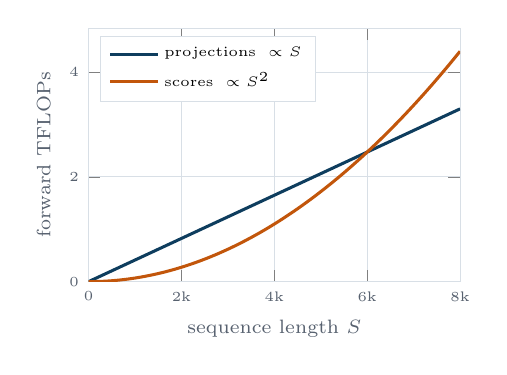
\begin{tikzpicture}
        \begin{axis}[
          width=6.3cm, height=4.8cm,
          xlabel={\scriptsize sequence length $S$},
          ylabel={\scriptsize forward TFLOPs},
          xmin=0,xmax=8192, ymin=0,
          xtick={0,2048,4096,6144,8192},
          xticklabels={0,2k,4k,6k,8k},
          tick label style={font=\tiny,color=nxSlate},
          label style={font=\tiny,color=nxSlate},
          axis line style={color=nxRule},
          grid=major, grid style={color=nxRule,line width=0.3pt},
          legend style={font=\tiny,draw=nxRule,at={(0.03,0.97)},
                        anchor=north west,fill=white},
          legend cell align=left,
        ]
        % One 4096-wide layer, 32 heads of 128: projections linear in S, the
        % score matrices quadratic. Four matmul terms each, 2 FLOP per MAC.
        \addplot[nxDeep,line width=1.1pt,domain=0:8192,samples=60,smooth]
          {4*3*2*x*4096*4096/1e12};
        \addlegendentry{projections $\;\propto S$}
        \addplot[nxFlame,line width=1.1pt,domain=0:8192,samples=60,smooth]
          {4*(4*32*x*x*128)/1e12};
        \addlegendentry{scores $\;\propto S^2$}
        \end{axis}
      \end{tikzpicture}
      \end{center}
      \begin{center}
      \begin{minipage}{0.94\linewidth}
        {\tiny\color{nxSlate}One 4096-wide layer. The crossing point is where
        context length stops being free --- worth answering before training,
        not after.}
      \end{minipage}
      \end{center}
    \end{column}
  \end{columns}
\end{frame}

\begin{frame}{The formula library}{Fifty-five layer types, each an independently checkable pure function}
  \vspace{0.3cm}
  \begin{center}
  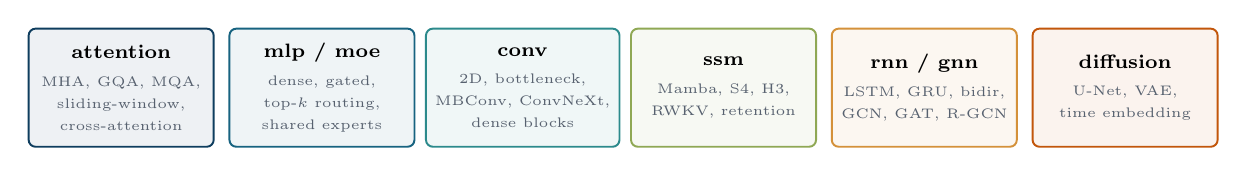
\begin{tikzpicture}[font=\scriptsize,
      f/.style={draw,rounded corners=2.5pt,minimum height=1.5cm,
                minimum width=2.35cm,align=center,line width=0.7pt}]
    \node[f,draw=ph1,fill=ph1!7]  (a) at (0,0)    {\textbf{attention}\\[2pt]\tiny\color{nxSlate}MHA, GQA, MQA,\\\tiny\color{nxSlate}sliding-window,\\\tiny\color{nxSlate}cross-attention};
    \node[f,draw=ph3,fill=ph3!7]  (b) at (2.55,0) {\textbf{mlp / moe}\\[2pt]\tiny\color{nxSlate}dense, gated,\\\tiny\color{nxSlate}top-$k$ routing,\\\tiny\color{nxSlate}shared experts};
    \node[f,draw=ph5,fill=ph5!7]  (c) at (5.10,0) {\textbf{conv}\\[2pt]\tiny\color{nxSlate}2D, bottleneck,\\\tiny\color{nxSlate}MBConv, ConvNeXt,\\\tiny\color{nxSlate}dense blocks};
    \node[f,draw=ph7,fill=ph7!7]  (d) at (7.65,0) {\textbf{ssm}\\[2pt]\tiny\color{nxSlate}Mamba, S4, H3,\\\tiny\color{nxSlate}RWKV, retention};
    \node[f,draw=ph9,fill=ph9!7]  (e) at (10.2,0) {\textbf{rnn / gnn}\\[2pt]\tiny\color{nxSlate}LSTM, GRU, bidir,\\\tiny\color{nxSlate}GCN, GAT, R-GCN};
    \node[f,draw=ph10,fill=ph10!7](f) at (12.75,0){\textbf{diffusion}\\[2pt]\tiny\color{nxSlate}U-Net, VAE,\\\tiny\color{nxSlate}time embedding};
  \end{tikzpicture}
  \end{center}

  \vspace{0.55cm}
  \begin{columns}[T]
    \begin{column}{0.48\textwidth}
      {\bfseries Pure, by construction}\\[5pt]
      \subtle{No state, no context, no I/O. \code{attention\_flops(B,S,H,h,causal)}
      returns the same number today and in a year. That is what makes each one
      checkable against a published count in isolation.}
    \end{column}
    \begin{column}{0.48\textwidth}
      {\bfseries Precision is a parameter, not a footnote}\\[5pt]
      \subtle{\code{dtype\_bytes} returns \code{f64}, not an integer, because
      int4 packs two values per byte. Returning 1 reported int4 as costing the
      same as int8 --- twice its real footprint, for exactly the quantisation
      people reach for to save memory.}
    \end{column}
  \end{columns}
\end{frame}

\begin{frame}{Phase 6: Memory}{Four terms, and the one everybody forgets}
  \vspace{0.1cm}
  \begin{columns}[T]
    \begin{column}{0.44\textwidth}
      \vspace{0.15cm}
      {\footnotesize
      \[ M_{\text{peak}} = \underbrace{P b}_{\text{params}}
                        + \underbrace{A}_{\text{activations}}
                        + \underbrace{P b}_{\text{gradients}}
                        + \underbrace{k P}_{\text{optimizer}} \]}
      \vspace{0.05cm}

      \subtle{$P$ parameters, $b$ bytes per element, $k$ the optimizer's state
      multiplier --- Adam keeps two moments in fp32, so $k = 8$ bytes per
      parameter whatever the training precision.}

      \vspace{0.3cm}
      \keypoint{\footnotesize A 7B model in bf16 is 14\,GB of weights and
      \emph{70\,GB} of training state. Sizing a run from the weight count
      alone is how a job dies at step one on a card that looked ample.}
    \end{column}
    \begin{column}{0.54\textwidth}
      \begin{center}
      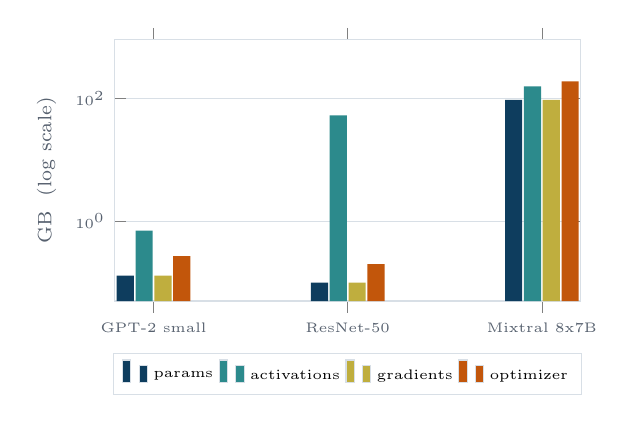
\begin{tikzpicture}
        \begin{axis}[
          width=7.5cm,height=4.9cm,
          % Grouped, not stacked: these are plotted on a log axis, and heights
          % on a log axis do not add. A stacked bar there would draw a total
          % that is not the sum of its parts.
          ybar=0.6pt, bar width=6.2pt,
          symbolic x coords={GPT-2 small,ResNet-50,Mixtral 8x7B},
          xtick=data, xticklabel style={font=\tiny,color=nxSlate},
          ylabel={\scriptsize GB \ (log scale)},
          ymode=log, log origin=infty, ymin=0.05, ymax=900,
          tick label style={font=\tiny,color=nxSlate},
          label style={font=\tiny,color=nxSlate},
          axis line style={color=nxRule},
          ymajorgrids, grid style={color=nxRule,line width=0.3pt},
          legend style={font=\tiny,draw=nxRule,at={(0.5,-0.20)},
                        anchor=north,legend columns=4,fill=white},
          legend cell align=left,
        ]
        \addplot[fill=ph1,draw=none] coordinates
          {(GPT-2 small,0.13) (ResNet-50,0.10) (Mixtral 8x7B,94.78)};
        \addlegendentry{params}
        \addplot[fill=ph5,draw=none] coordinates
          {(GPT-2 small,0.70) (ResNet-50,52.95) (Mixtral 8x7B,156.23)};
        \addlegendentry{activations}
        \addplot[fill=ph8,draw=none] coordinates
          {(GPT-2 small,0.13) (ResNet-50,0.10) (Mixtral 8x7B,94.78)};
        \addlegendentry{gradients}
        \addplot[fill=ph10,draw=none] coordinates
          {(GPT-2 small,0.27) (ResNet-50,0.20) (Mixtral 8x7B,189.55)};
        \addlegendentry{optimizer}
        \end{axis}
      \end{tikzpicture}
      \end{center}
      \begin{center}
      \begin{minipage}{0.95\linewidth}
        {\tiny\color{nxSlate}Computed by NEURAX. Peak: 1.24, 53.4, 535\,GB.}
      \end{minipage}
      \end{center}
    \end{column}
  \end{columns}
\end{frame}

\begin{frame}{Phase 7: Parallelism}{What happens when one device is not enough}
  \vspace{0.15cm}
  \begin{columns}[T]
    \begin{column}{0.46\textwidth}
      {\bfseries Sharding}\\[4pt]
      \subtle{ZeRO stages 0--3 progressively shard the optimizer state, then the
      gradients, then the parameters themselves. Each stage reduces memory per
      device and changes what has to be communicated.}\\[9pt]

      {\bfseries Communication}\\[4pt]
      \subtle{A data-parallel step must all-reduce one buffer the size of the
      gradients --- not the model's whole memory traffic. ZeRO-3 in particular
      \emph{increases} communication: it must gather sharded parameters back on
      demand.}\\[9pt]

      \keypoint{\footnotesize Scaling efficiency is derived, not assumed. The
      pass reports the GPU count past which adding hardware stops buying time.}
    \end{column}
    \begin{column}{0.5\textwidth}
      \begin{center}
      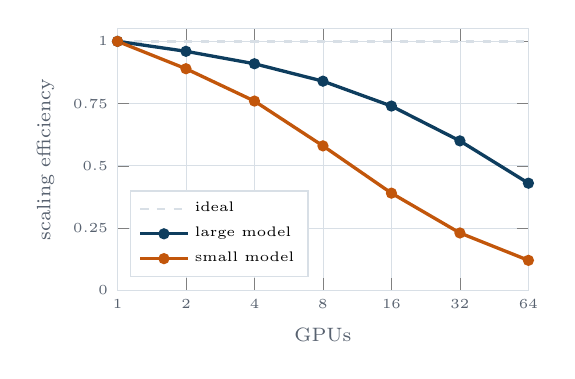
\begin{tikzpicture}
        \begin{axis}[
          width=6.8cm,height=4.9cm,
          xlabel={\scriptsize GPUs}, ylabel={\scriptsize scaling efficiency},
          xmin=1,xmax=64,ymin=0,ymax=1.05,
          xmode=log, log basis x=2,
          xtick={1,2,4,8,16,32,64},
          xticklabels={1,2,4,8,16,32,64},
          ytick={0,0.25,0.5,0.75,1.0},
          tick label style={font=\tiny,color=nxSlate},
          label style={font=\tiny,color=nxSlate},
          axis line style={color=nxRule},
          grid=major, grid style={color=nxRule,line width=0.3pt},
          legend style={font=\tiny,draw=nxRule,at={(0.03,0.05)},
                        anchor=south west,fill=white},
          legend cell align=left,
        ]
        \addplot[nxRule,line width=0.9pt,dashed,domain=1:64,samples=2] {1};
        \addlegendentry{ideal}
        \addplot[nxDeep,line width=1.2pt,mark=*,mark size=1.4pt]
          coordinates {(1,1.0)(2,0.96)(4,0.91)(8,0.84)(16,0.74)(32,0.60)(64,0.43)};
        \addlegendentry{large model}
        \addplot[nxFlame,line width=1.2pt,mark=*,mark size=1.4pt]
          coordinates {(1,1.0)(2,0.89)(4,0.76)(8,0.58)(16,0.39)(32,0.23)(64,0.12)};
        \addlegendentry{small model}
        \end{axis}
      \end{tikzpicture}
      \end{center}
      \vspace{-0.1cm}
      \subtle{\tiny Shape of the curve the pass produces: communication is a fixed
      cost per step, so the smaller the compute per device, the sooner it
      dominates. Illustrative shape; the pass computes the real curve per model.}
    \end{column}
  \end{columns}
\end{frame}

\begin{frame}{Phase 8: Hardware}{The roofline --- and why latency is not simply the larger of two numbers}
  \vspace{0.1cm}
  \begin{columns}[T]
    \begin{column}{0.47\textwidth}
      \begin{center}
      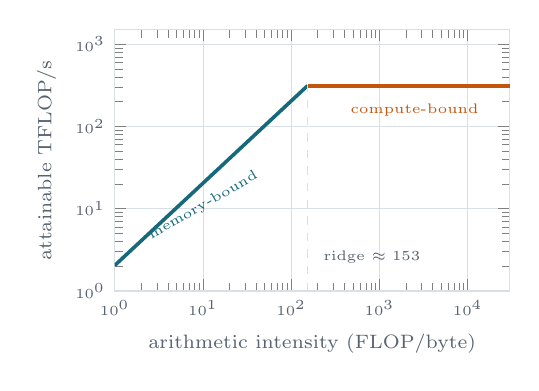
\begin{tikzpicture}
        \begin{axis}[
          width=6.6cm,height=4.9cm,
          xlabel={\scriptsize arithmetic intensity (FLOP/byte)},
          ylabel={\scriptsize attainable TFLOP/s},
          xmode=log, ymode=log,
          xmin=1, xmax=30000, ymin=1, ymax=1500,
          tick label style={font=\tiny,color=nxSlate},
          label style={font=\tiny,color=nxSlate},
          axis line style={color=nxRule},
          grid=major, grid style={color=nxRule,line width=0.3pt},
        ]
        % Memory roof: 2039 GB/s is 2.039 TFLOP/s per FLOP/byte.
        \addplot[nxTeal,line width=1.3pt] coordinates {(1,2.039)(153,312)};
        % Compute roof: 312 TFLOP/s fp16, flat once the ridge is passed.
        \addplot[nxFlame,line width=1.3pt] coordinates {(153,312)(30000,312)};
        \draw[nxRule,dashed,line width=0.7pt]
          (axis cs:153,1) -- (axis cs:153,312);
        \node[font=\tiny,color=nxSlate,anchor=west] at (axis cs:180,2.6)
          {ridge $\approx 153$};
        \node[font=\tiny,color=nxTeal,anchor=west,rotate=30] at (axis cs:2,4)
          {memory-bound};
        \node[font=\tiny,color=nxFlame,anchor=north] at (axis cs:2500,250)
          {compute-bound};
        \end{axis}
      \end{tikzpicture}
      \end{center}
      \vspace{0.1cm}
      \begin{center}
      \begin{minipage}{0.95\linewidth}
        {\tiny\color{nxSlate}A100-80GB: 312 TFLOP/s fp16, 2039 GB/s. NEURAX
        computes the ridge as
        $\text{peak}\times\text{efficiency}\,/\,\text{bandwidth}$.}
      \end{minipage}
      \end{center}
    \end{column}
    \begin{column}{0.5\textwidth}
      {\bfseries Latency, as modelled}\\[3pt]
      {\footnotesize
      \[ t = \max(t_c,t_m) + \min(t_c,t_m)(1-\rho) + t_{\text{comm}} + n_k \tau \]}
      \vspace{-0.1cm}

      \subtle{$t_c$ compute, $t_m$ memory, $\rho$ overlap, $n_k$ kernels,
      $\tau$ per-launch overhead.}

      \vspace{0.18cm}
      \keypoint{\scriptsize Taking $\max(t_c,t_m)$ alone assumes compute and
      memory overlap perfectly. No real GPU does. NEURAX uses $\rho = 0.3$ and
      adds $5\,\mu\text{s}$ per kernel launch --- for a model issuing
      thousands of small kernels, not a rounding error.\\[4pt]
      Bottlenecks carry a dead band too: compute- or memory-bound only past
      $1.5\times$, otherwise \emph{balanced}.}
    \end{column}
  \end{columns}
\end{frame}

\begin{frame}{Phases 9--10: Cost and Report}{Where FLOPs become hours, money, kilowatt-hours and carbon}
  \vspace{0.25cm}
  \begin{center}
  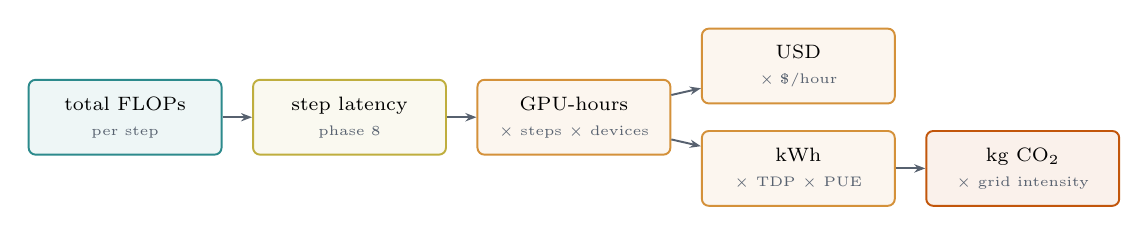
\begin{tikzpicture}[font=\scriptsize,
      s/.style={draw,rounded corners=2.5pt,minimum height=0.95cm,
                minimum width=2.45cm,align=center,line width=0.7pt}]
    \node[s,draw=ph5,fill=ph5!8]  (f) at (0,0)     {total FLOPs\\[1pt]\tiny\color{nxSlate}per step};
    \node[s,draw=ph8,fill=ph8!8]  (t) at (2.85,0)  {step latency\\[1pt]\tiny\color{nxSlate}phase 8};
    \node[s,draw=ph9,fill=ph9!8]  (h) at (5.70,0)  {GPU-hours\\[1pt]\tiny\color{nxSlate}$\times$ steps $\times$ devices};
    \node[s,draw=ph9,fill=ph9!8]  (m) at (8.55,0.65) {USD\\[1pt]\tiny\color{nxSlate}$\times$ \$/hour};
    \node[s,draw=ph9,fill=ph9!8]  (e) at (8.55,-0.65) {kWh\\[1pt]\tiny\color{nxSlate}$\times$ TDP $\times$ PUE};
    \node[s,draw=ph10,fill=ph10!8](c) at (11.4,-0.65) {kg CO$_2$\\[1pt]\tiny\color{nxSlate}$\times$ grid intensity};

    \foreach \a/\b in {f/t,t/h}
      \draw[-{Stealth[length=4pt]},nxSlate,line width=0.7pt] (\a) -- (\b);
    \draw[-{Stealth[length=4pt]},nxSlate,line width=0.7pt] (h) -- (m);
    \draw[-{Stealth[length=4pt]},nxSlate,line width=0.7pt] (h) -- (e);
    \draw[-{Stealth[length=4pt]},nxSlate,line width=0.7pt] (e) -- (c);
  \end{tikzpicture}
  \end{center}

  \vspace{0.4cm}
  \begin{columns}[T]
    \begin{column}{0.48\textwidth}
      {\bfseries The report is not a formatting step}\\[5pt]
      \subtle{It assembles every pass's metrics into one document and runs the
      diagnostic rules across the whole picture --- checks that need more than
      one pass's output to be possible.}
    \end{column}
    \begin{column}{0.48\textwidth}
      {\bfseries Diagnostics carry a code and a suggestion}\\[5pt]
      \subtle{\code{E001--E005} errors, \code{W001--W009} warnings,
      \code{H001--H008} hints, \code{I001--I003} information. Each has a
      severity, an optional layer to point at, and an estimate of its impact on
      the report's own precision.}
    \end{column}
  \end{columns}
\end{frame}

\begin{frame}{Phase 11: Dynamic analysis}{Three questions that are about behaviour rather than arithmetic}
  \vspace{0.35cm}
  \begin{columns}[T]
    \begin{column}{0.30\textwidth}
      \phasebadge{ph11}{VIRTUAL MEMORY}\\[8pt]
      \subtle{Allocation behaviour over a step: liveness intervals, the
      fragmentation a real allocator would suffer, and the largest batch that
      still fits.}
    \end{column}
    \begin{column}{0.30\textwidth}
      \phasebadge{ph11}{STABILITY}\\[8pt]
      \subtle{Numerical risk read off the graph and the precision: depth without
      normalisation, activation ranges that overflow fp16, initialisation that
      will not hold across the reported depth.}
    \end{column}
    \begin{column}{0.30\textwidth}
      \phasebadge{ph11}{BEHAVIOURAL}\\[8pt]
      \subtle{Synthesises the step profile from the compute IR --- which
      operations dominate, and what the shape of a step actually looks like.}
    \end{column}
  \end{columns}

  \vspace{0.7cm}
  \keypoint{Its stability output feeds a hyperparameter hint in the report
  (\code{H007}), which is why it must finish before the report is closed ---
  but it reads neither cost nor hardware, so it does not have to wait for them.}
\end{frame}

\begin{frame}{The compiler's own dependency graph}{Eleven passes, but not eleven serial steps}
  \vspace{0.3cm}
  \begin{center}
  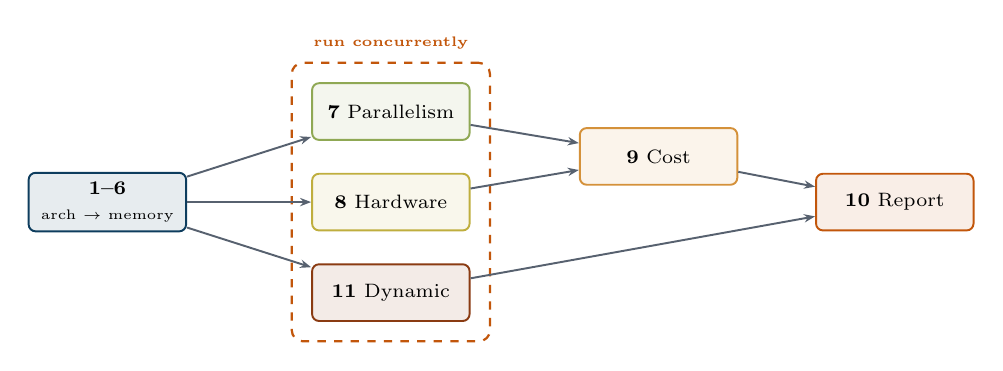
\begin{tikzpicture}[font=\scriptsize,
      b/.style={draw,rounded corners=2.5pt,minimum height=0.72cm,
                minimum width=2.0cm,align=center,line width=0.7pt,
                font=\scriptsize}]
    \node[b,draw=ph1,fill=ph1!10] (chain) at (0,0)
      {\textbf{1--6}\\[1pt]\tiny arch $\rightarrow$ memory};

    \node[b,draw=ph7,fill=ph7!10]  (par) at (3.6,1.15) {\textbf{7} Parallelism};
    \node[b,draw=ph8,fill=ph8!10]  (hw)  at (3.6,0)    {\textbf{8} Hardware};
    \node[b,draw=ph11,fill=ph11!10](dyn) at (3.6,-1.15){\textbf{11} Dynamic};

    \node[b,draw=ph9,fill=ph9!10]  (cost) at (7.0,0.58) {\textbf{9} Cost};
    \node[b,draw=ph10,fill=ph10!10](rep)  at (10.0,0)   {\textbf{10} Report};

    \foreach \t in {par,hw,dyn}
      \draw[-{Stealth[length=4pt]},nxSlate,line width=0.7pt] (chain) -- (\t);
    \draw[-{Stealth[length=4pt]},nxSlate,line width=0.7pt] (par) -- (cost);
    \draw[-{Stealth[length=4pt]},nxSlate,line width=0.7pt] (hw) -- (cost);
    \draw[-{Stealth[length=4pt]},nxSlate,line width=0.7pt] (cost) -- (rep);
    \draw[-{Stealth[length=4pt]},nxSlate,line width=0.7pt] (dyn) -- (rep);

    \begin{scope}[on background layer]
      \node[draw=nxFlame,dashed,rounded corners=4pt,line width=0.8pt,
            fit=(par)(hw)(dyn),inner sep=7pt] (grp) {};
    \end{scope}
    \node[above=1pt of grp,text=nxFlame,font=\tiny\bfseries] {run concurrently};
  \end{tikzpicture}
  \end{center}

  \vspace{0.45cm}
  \keypoint{Phases 7, 8 and 11 read only what phases 1--6 produced, and nothing
  from each other --- so they run in parallel. Dynamic analysis used to wait for
  Cost and Report even though it never touches their output: dead
  serialisation, removed by reading the dependency graph rather than the phase
  numbering.}
\end{frame}

% =====================================================================
\section{Validation}
% =====================================================================

\begin{frame}{Does it agree with reality?}{Eleven reference models against their published parameter counts}
  \vspace{0.15cm}
  \begin{center}
  {\footnotesize
  \begin{tabular}{@{}l r r r@{}}
    \toprule
    \textbf{Model} & \textbf{Published} & \textbf{NEURAX} & \textbf{Error} \\
    \midrule
    GCN (ogbn-arxiv) & 110\,120 & 110\,120 & \good{$+0.00\%$} \\
    DCGAN            & 6.342\,M & 6.340\,M & \good{$-0.03\%$} \\
    ResNet-50        & 25.6\,M  & 25.59\,M & \good{$-0.04\%$} \\
    GPT-3 175B       & 175.0\,B & 174.6\,B & \good{$-0.24\%$} \\
    VGG-16           & 138\,M   & 138.4\,M & \good{$+0.26\%$} \\
    AWD-LSTM (PTB)   & 24\,M    & 24.20\,M & \good{$+0.84\%$} \\
    Mixtral 8$\times$7B & 46.7\,B & 47.39\,B & \good{$+1.47\%$} \\
    LLaMA-2 70B      & 70.0\,B  & 68.72\,B & \good{$-1.82\%$} \\
    RWKV-4 7B        & 7.5\,B   & 7.19\,B  & $-4.17\%$ \\
    Mamba 2.8B       & 2.8\,B   & 2.66\,B  & $-4.89\%$ \\
    DeepSeek-V3      & 671\,B   & 701.4\,B & $+4.53\%$ \\
    \bottomrule
  \end{tabular}}
  \end{center}

  \vspace{0.25cm}
  \begin{center}\begin{minipage}{0.88\linewidth}
    {\scriptsize\color{nxSlate}Sources cited per row in the test itself:
    papers where a count is published, independent re-derivation where it is
    not. Published counts are themselves approximate --- they disagree on tied
    embeddings and on whether biases are counted.}
  \end{minipage}\end{center}
\end{frame}

\begin{frame}{The test that found four wrong answers}{Written to check the thing it claimed to check}
  \vspace{0.2cm}
  \begin{center}
  {\footnotesize
  \begin{tabular}{@{}l r r r@{}}
    \toprule
    \textbf{Model} & \textbf{Published} & \textbf{First measured} & \textbf{Error} \\
    \midrule
    LLaMA-2 70B         & 70.0\,B  & 49.9\,B   & \bad{$-28.7\%$} \\
    Mixtral 8$\times$7B & 46.7\,B  & 103.8\,B  & \bad{$+122\%$} \\
    DeepSeek-V3         & 671\,B   & 1\,395\,B & \bad{$+108\%$} \\
    RWKV 7B             & 7.5\,B   & 0.24\,B   & \bad{$-96.7\%$} \\
    \bottomrule
  \end{tabular}}
  \end{center}

  \vspace{0.5cm}
  \begin{columns}[T]
    \begin{column}{0.55\textwidth}
      {\bfseries Three causes, all structural}\\[6pt]
      \subtle{$\bullet$ A scale derived from the attention-block count was applied
      to \emph{every} repeating kind, so a config listing 2 attention and 4
      mixture blocks got twice the mixture layers it asked for.}\\[4pt]
      \subtle{$\bullet$ \code{shared\_experts} defaulted to 1, adding an expert to
      every mixture that never mentioned one.}\\[4pt]
      \subtle{$\bullet$ RWKV was costed with Mamba's formula.}
    \end{column}
    \begin{column}{0.41\textwidth}
      \keypoint{\footnotesize A test named
      \code{modelTemplates.accuracy.test.ts} claimed these models ``must
      reproduce their published parameter counts''. It checked parameter
      \emph{name aliasing}. Nothing anywhere compared a computed figure to a
      known one --- so all four errors were invisible while the suite was
      green.}
    \end{column}
  \end{columns}
\end{frame}

\begin{frame}{What it costs to ask}{One machine, release build, best of 25 runs each}
  \vspace{0.15cm}
  \begin{center}
  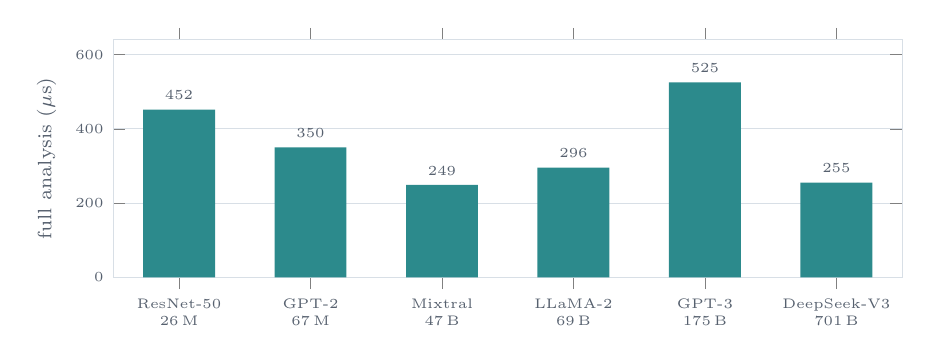
\begin{tikzpicture}
    \begin{axis}[
      width=11.6cm,height=4.6cm,
      ybar, bar width=26pt,
      symbolic x coords={ResNet-50,GPT-2,Mixtral,LLaMA-2,GPT-3,DeepSeek-V3},
      xticklabels={ResNet-50\\{\tiny 26\,M},GPT-2\\{\tiny 67\,M},%
                   Mixtral\\{\tiny 47\,B},LLaMA-2\\{\tiny 69\,B},%
                   GPT-3\\{\tiny 175\,B},DeepSeek-V3\\{\tiny 701\,B}},
      xticklabel style={align=center},
      xtick=data, xticklabel style={font=\tiny,color=nxSlate},
      ylabel={\scriptsize full analysis ($\mu$s)},
      ymin=0,ymax=640,
      nodes near coords, nodes near coords style={font=\tiny,color=nxSlate},
      tick label style={font=\tiny,color=nxSlate},
      label style={font=\tiny,color=nxSlate},
      axis line style={color=nxRule},
      ymajorgrids, grid style={color=nxRule,line width=0.3pt},
    ]
    \addplot[fill=ph5,draw=none] coordinates
      {(ResNet-50,452) (GPT-2,350) (Mixtral,249)
       (LLaMA-2,296) (GPT-3,525) (DeepSeek-V3,255)};
    \end{axis}
  \end{tikzpicture}
  \end{center}

  \vspace{0.2cm}
  \keypoint{\footnotesize A 701-billion-parameter model is analysed in
  \term{255 microseconds} --- faster than a 26-million-parameter one. Cost
  tracks the number of \emph{layer definitions}, not parameters, because
  nothing is ever allocated.}
\end{frame}

% =====================================================================
\section{Limits}
% =====================================================================

\begin{frame}{What the compiler does not know}{Stated here so it is not discovered later}
  \vspace{0.3cm}
  \begin{columns}[T]
    \begin{column}{0.47\textwidth}
      {\color{nxRose}\bfseries Outside the model entirely}\\[6pt]
      \textcolor{nxRule}{\rule{\linewidth}{0.6pt}}\\[8pt]
      \begin{itemize}\setlength\itemsep{6pt}
        \item[] \subtle{\textbf{Convergence.} It reports what a step costs, never
        whether the model learns. No accuracy, no loss curve.}
        \item[] \subtle{\textbf{Kernel scheduling.} Real occupancy, cache
        behaviour and launch ordering are represented by two constants, not
        simulated.}
        \item[] \subtle{\textbf{Framework overhead.} Python, the data loader, and
        checkpoint I/O are not in the model.}
      \end{itemize}
    \end{column}
    \begin{column}{0.47\textwidth}
      {\color{nxFlame}\bfseries Approximations it makes on purpose}\\[6pt]
      \textcolor{nxRule}{\rule{\linewidth}{0.6pt}}\\[8pt]
      \begin{itemize}\setlength\itemsep{6pt}
        \item[] \subtle{\textbf{Backward $= 2\times$ forward.} Standard, and wrong
        in the third digit for architectures with heavy recomputation.}
        \item[] \subtle{\textbf{Optimizer $\approx 10\%$.} A constant, not a
        derivation.}
        \item[] \subtle{\textbf{Efficiency factors.} Per-operation, per-device
        multipliers from a calibration table --- the one place measured data
        enters the model.}
      \end{itemize}
    \end{column}
  \end{columns}

  \vspace{0.25cm}
  \keypoint{\footnotesize These are the boundary of the claim, not caveats in
  a footnote. The compiler answers ``what will this cost'', to a few percent,
  in microseconds. It does not answer ``will this work''.}
\end{frame}

\begin{frame}{In summary}{}
  \vspace{0.5cm}
  \begin{columns}[T]
    \begin{column}{0.48\textwidth}
      {\Large\color{nxDeep}\bfseries The compiler}\\[10pt]
      \begin{itemize}\setlength\itemsep{7pt}
        \item Eleven dialects, from a JSON architecture to a costed report
        \item Every pass builds, measures and \emph{validates} before the next
        one may read it
        \item Fifty-five layer types, as pure functions checkable in isolation
        \item Nothing is ever executed --- no tensor, no kernel, no weight
      \end{itemize}
    \end{column}
    \begin{column}{0.48\textwidth}
      {\Large\color{nxFlame}\bfseries What that buys}\\[10pt]
      \begin{itemize}\setlength\itemsep{7pt}
        \item Parameter counts within a few percent of eleven published models
        \item A full analysis in a few hundred microseconds, at any model size
        \item Answers before the hardware is provisioned, not after
        \item A cost that can be swept across thousands of configurations
      \end{itemize}
    \end{column}
  \end{columns}

  \vspace{0.9cm}
  \begin{center}
    \textcolor{nxRule}{\rule{0.5\linewidth}{0.8pt}}\\[10pt]
    {\large\color{nxInk}Know what it costs while it is still a question.}
  \end{center}
\end{frame}

\end{document}
